\documentclass[tikz]{standalone}
\usepackage{ctex}
\usepackage{tikz}
\usepackage{pgfplots}
\pgfplotsset{compat=1.18}   % 使用较新版本语法
\usetikzlibrary{positioning, arrows.meta, intersections, calc, fit, backgrounds}
\usepgfplotslibrary{fillbetween}  % 用于填充区域

\begin{document}

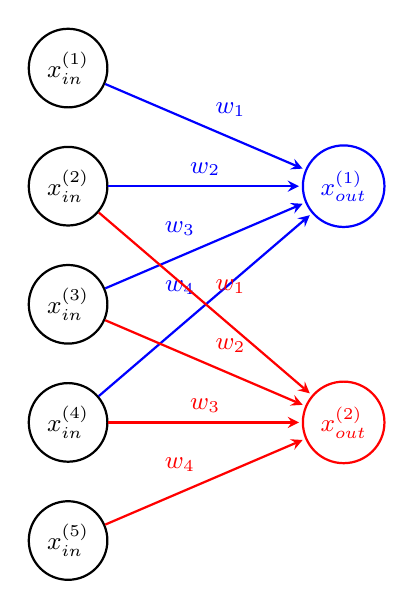
\begin{tikzpicture}[->,>=stealth,shorten >=1pt,auto,node distance=1.5cm,
    thick,main node/.style={circle,draw,font=\sffamily\small}]

    \node[main node] (a) {$x_\text{in}^{(1)}$};
    \node[main node] (b) [below of=a] {$x_\text{in}^{(2)}$};
    \node[main node] (c) [below of=b] {$x_\text{in}^{(3)}$};
    \node[main node] (d) [below of=c] {$x_\text{in}^{(4)}$};
    \node[main node] (e) [below of=d] {$x_\text{in}^{(5)}$};

    \node[main node,draw=blue,text=blue] (f) [right of=b, xshift=2cm] {$x_\text{out}^{(1)}$};
    \node[main node,draw=red, text=red] (g) [right of=d, xshift=2cm] {$x_\text{out}^{(2)}$};

    \path[every node/.style={font=\sffamily\small}]
    (a) edge[draw=blue] node [bend left,text=blue] {$w_1$} (f)
    (b) edge[draw=blue] node [bend left,text=blue] {$w_2$} (f)
    (c) edge[draw=blue] node [bend left,text=blue] {$w_3$} (f)
    (d) edge[draw=blue] node [bend left,text=blue] {$w_4$} (f)
    (b) edge[draw=red] node [bend right,text=red] {$w_1$} (g)
    (c) edge[draw=red] node [bend right,text=red] {$w_2$} (g)
    (d) edge[draw=red] node [bend right,text=red] {$w_3$} (g)
    (e) edge[draw=red] node [bend right,text=red] {$w_4$} (g);
\end{tikzpicture}
\end{document}